\chapter{Design}
\label{chap:Design}
%\funnyquote{Il semble que la perfection soit atteinte non quand il n'y a plus
%rien \`a ajouter, mais quand il n'y a plus rien \`a retrancher.}
%{Antoine de Saint-Exup\'ery}
%
%\funnyquote{It can scarcely be denied that the supreme goal of all theory is to
%make the irreducible basic elements as simple and as few as possible without
%having to surrender the adequate representation of a single datum of
%experience.}
%{Albert Einstein}
%
\funnyquote{There are only two kinds of languages: the ones people complain
about and the ones nobody uses.}
{Bjarne Stroustrup~\footnote{\textit{Of course, all "there are only
two" quotes have to be taken with a grain of salt.}~\cite{stroustrup}}}


In this chapter, we elaborate on the design of the message-sending and
object-representation layers because they are the key components of Photon's
runtime environment. As introduced previously, the former is the primitive used
to reify low-level operations and the latter serves to efficiently isolate the
application from the instrumentation code.  We first introduce the semantics of
the message-sending operation and discuss its efficient implementation. We then
introduce our object representation, which takes advantage of the method
invocation optimizations performed by the underlying VM. Finally, a brief
compilation example is provided to illustrate how JavaScript can be compiled to
this runtime environment.

\section{Message-sending foundation}
In our design, the message-sending operation serves to unify all reified
operations, namely operations on objects and function calls, around a single
mechanism. It facilitates the achievement of correctness, because a single
primitive operation needs to be added to the implementation, and performance,
because its implementation targets the highest performing operations of the
underlying system.  The particular choice of message-sending as a foundation
was motivated by its tried and true application to Smalltalk and Self with
success for the obtention of a dynamic, open and fast implementation. 

% Open, Dynamic
\subsection{Semantics}

We now see the chosen semantics for the message-sending operation, in steps. We
first discuss the basic operation, that closely corresponds to a method call in
JavaScript. We  then reify the function call to allow its redefinition. We then
reify the memoization operation performed by inline caches to enable functions
to specify their cached behavior. 

The implementation of message sends uses our object representation but could
accomodate other representation choices. Our object representation will be
fully explained in the next section. For now, it is sufficient to think of our
representation as proxies to native objects with methods for reified operations
that provide isolation and encapsulate low-level details necessary for
optimization. This section uses the following methods:
\begin{itemize}
    \item \kw{call(rcv, ..args)}: calls the object as a method with the
    \kw{rcv} receiver and \kw{args} arguments and returns its return value
    \item \kw{get(name)}: returns the value of the \kw{name} property on
    this object and implicitly performs a lookup on the prototype chain
    \item \kw{unbox()}: returns the native object wrapped by the representation 
\end{itemize}

Unless specified, the pseudo-code follows the regular JavaScript semantics.
For presentation simplicity, we use the rest and spread operators
(\kw{..args}), to appear in the next version of JavaScript~\cite{ECMAScript6},
and  we omit primitive values, missing values and error handling.

\subsubsection{Message sending as a method call}

The basic version essentially performs a regular lookup followed by a call to
the function retrieved with the receiver object. This corresponds to the
semantics of a method call in JavaScript:

\jsfile{listings/basic-send.js}


\subsubsection{Reifying function calls}
\label{sec:AugmentedFunctionCalling}

In JavaScript, the \kw{call} method on every function reifies the calling
protocol and allows a program to call into a function at run time, as if it was
done through the direct mechanisms. The exact behavior of a function call
should be the same, whether it is called directly or indirectly. However, there
is no causal connection between the state of the \kw{call} method and the
behavior of function calls. In other words, redefining the \kw{call} method on
\kw{Function.prototype} does not affect the behavior of call sites.

We can establish this causal relationship with a slight modification of the
send operation:

\jsfile{listings/augmented-send.js}

This semantics allows a particular function to be instrumented, simply by
redefining its call method.

\subsubsection{Providing a memoization hook}

When designing an instrumentation framework, a choice in the granularity of
instrumentation needs to be made. For example, a corse-grained design would use
a single method implementation for all operation call sites. For Photon, we
chose a fine-grained design, where the implementation of every call site can be
different. An operation, instrumented or not, is specialized with the
information available at the call site. We expose this functionality to
instrumentation writers through a special \kw{\_\_memoize\_\_} method, specific
to each reified operation.

Our mechanism allows a method to inspect its arguments and receiver to
specialize itself for subsequent calls. The first call is always performed by
calling the original function while all subsequent calls are made to the
memoized function. A \kw{\_\_memoize\_\_} method on a reified operation is
called the first time the operation is invoked to provide the specialized
method that will be used on all subsequent calls.

There is an unfortunate interaction between memoization and the reification of
the call protocol. Care must be taken because memoization can only occur if the
call method of the function has not been redefined. Otherwise, the identity of
the function passed to the call method would not be the same. To preserve
identity while allowing memoization, the behavior of the cache can be different
depending on the state of the \kw{Function.prototype}'s \kw{call} method. If its
value is the default one, the identity of the function is not important and
memoization can be performed. Otherwise, memoization is ignored.

The extended semantics, including memoization at the call site is the
following:

\jsfile{listings/memoized-send.js}

\subsection{Translating reified operations to message-sending}

Reifying object operations and function calls is done by translation to
corresponding message sends. Table~\ref{tb:CallTypes} summarizes all the
different source code occurrences of calls and their equivalent message sends
and Table~\ref{tb:ObjectModelOperations} explains the translations for object
operations.

\begin{table}[htb]
\caption{Call types and their equivalent message sends}
\centering

\begin{tabular}{|p{.25\textwidth}|p{.33\textwidth}|p{.33\textwidth}|}
  \hline
  Call Type & Explanation & Equivalent Message Send \\
  \hline \hline
    \tbbox{Global\\} & 
    \tbbox{
        Calling a function whose value is in a global variable. \\
        Ex: \kw{foo()}
    } &
    \tbbox{
        Sending a message to the global object. \\
        Ex: \kw{send(global,"foo")}
    } \\
  \hline
  \tbbox{Local\\} & 
    \tbbox{
        Calling a function in a local variable.  \\
        Ex: \kw{fn()}
    } &
    \tbbox{
        Sending the \kw{call} message to the function.\\
        Ex: \kw{send(fn,"call")}
    } \\
  \hline
  \tbbox{Method\\} & 
    \tbbox{
        Calling an object method. \\
        Ex: \kw{obj.foo()}
    } &
    \tbbox{
        Sending a message to the object.\\
        Ex: \kw{send(obj,"foo")}
    } \\
  \hline
  \tbbox{\kw{apply} or \kw{call}} & 
    \tbbox{
        Calling the \kw{call} or \kw{apply} function method. \\
        Ex: \kw{fn.call()}
    } &
    \tbbox{
        Sending the \kw{call} or \kw{apply} message.\\
        Ex: \kw{send(fn,"call")}
    } \\
  \hline
\end{tabular}

\label{tb:CallTypes}
\end{table}


\begin{table}[!hbt]
\caption{Object operations and their equivalent message sends}
\centering

\begin{tabular}{|p{.25\textwidth}|p{.32\textwidth}|p{.35\textwidth}|}
  \hline
  Object Model Operation & Explanation & Equivalent Message Send \\
  \hline \hline
  \tbbox{Property access} & 
    \tbbox{
        Retrieving the value of a property that might exist or not.\\
        Ex: \kw{obj.foo}  
    } &
    \tbbox{
        Sending the \kw{__get__} message.\\
        Ex: \kw{send(obj,"__get__","foo")}
    } \\
  \hline
  \tbbox{Property assignation} & 
    \tbbox{
        Creating or updating a property.\\
        Ex: \kw{obj.foo=42} 
    } &
    \tbbox{
        Sending the \kw{__set__} message.\\
        Ex: \kw{send(obj,"__set__","foo",42)}
    } \\
  \hline
  \tbbox{Property deletion} &
    \tbbox{
        Deleting a property that might exist or not.\\
        Ex: \kw{delete obj.foo}
    } &
    \tbbox{
        Sending the \kw{__delete__} message. Ex:\\
        \kw{send(obj,"__delete__","foo")}
    } \\
  \hline
  \tbbox{Object litteral creation} & 
    \tbbox{
        Creating an object in-place.\\
        Ex: \kw{\{foo:42\}} 
    } &
    \tbbox{
        Sending the \kw{__new__} message.\\
        Ex: \kw{send(\{foo:42\}, "__new__")}
    } \\
  \hline
  \tbbox{Constructor creation} & 
    \tbbox{
        Creating an object with \kw{new}. \\
        Ex: \kw{new Fun()}
    } &
    \tbbox{
        Sending the \kw{__ctor__} message.\\
        Ex: \kw{send(Fun, "__ctor__")}
    } \\
  \hline
\end{tabular}

\label{tb:ObjectModelOperations}
\end{table}

\subsection{Efficient implementation}
\label{sec:EfficientImplementation}

The reification of low-level operations of JS with message sends introduces a
performance penalty compared to a native execution. Our design takes advantage
of optimizations performed by the host VM to efficiently implement reified
operations.  The core insight behind our implementation comes from seeing
global function calls of the host VM both as an optimized calling mechanism and
as a dynamically specializable operation. They provide the same ability as code
patching in assembly. On the current version of V8, when the number of
arguments expected matches the number of arguments supplied, it opens the
possibility of inlining the function at the call site. If the global function
changes at a later time, the call site is deoptimized transparently. It
is a really powerful mechanism because much of the complexity of run-time
specialization is performed by the underlying host.  We can simply piggyback on
those optimizations.

To motivate the actual optimizing implementation, let's use the following
unoptimizing translation of a call to the method \kw{bar} on the object
\kw{obj} inside a function \kw{foo}:

\jsfile{listings/send-example.js}

Notice that by specializing the operation to the information available at its
call site, a more efficient version can be provided. In this example, the name
of the method is constant. If we further suppose that the \kw{call} method on
\kw{Function.prototype} has not been redefined, the implementation of a
message-send can be inlined and stripped of the generality required to reify
function calls. Using the memoization mechanism the resulting call site will be
specialized to the following implementation:

\jsfile{listings/inline-cache-optimized-example.js}

In Photon, this specialization is done at run time. Initially, the global
variable corresponding to the call site is initialized with a generic function
that will be replaced by the specialized version during the first call to the
reified operation. The next listing shows the actual implementation in the
initial state of the cache:

\jsfile{listings/inline-cache-example.js}

Executing the code will eventually replace \kw{codeCache0} with the expected
method, corresponding to the second return statement in the \kw{initState}
function.

\subsubsection{Cache states and transitions}

The previous section has shown two different states of a message send call
site, used to optimize subsequent calls to reified operations.  In this
section, we fully define the behaviors of the inline caches and the conditions
that trigger those behaviors.  We use a state machine formalism to present the
different behaviors associated with inline caches and the triggers that are
responsible for the transitions between those behaviors. In our formalism, due
to the nature of synchronous message sends, a state transition occurs before
the event has been fully processed. However, the processing of the event is not
influenced by it.  

To simplify the tracking of invariants, we decided to always perform lookups for
regular method calls. By making the lookup operation as close as possible to
the native operation of JavaScript, it allows the underlying VM to optimize it.
In our design, the idea is to delegate the regular method call to the object
representation. The other important operation was to allow specialization of
object model operations, which is critical for speed. This is done by memoizing
a specialized version in the inline cache. We therefore ended up with two
states in addition to the initial state of the cache, as explained in
table~\ref{tb:CacheStates}.

\begin{table}[htb]
\caption{Cache states}
\centering

\begin{tabular}{|p{.33\textwidth}|p{.33\textwidth}|}
  \hline
  Cache states & Explanation \\
  \hline \hline
  \tbbox{Initial State} & 
    \tbbox{
        Perform a regular send.
    } \\
  \hline
  \tbbox{Regular method call} & 
    \tbbox{
        Lookup method then call.
    } \\
  \hline
  \tbbox{Memoized method call} & 
    \tbbox{
        Method specific behavior. The memoized method is responsible for
        maintaining invariants.
    } \\
  \hline
\end{tabular}

\label{tb:CacheStates}
\end{table}


Transitions between states happen on message sends and object model operation
events.  An insight was to realize that we could underapproximate the tracking
of invariants and conservatively invalidate more caches than what would
minimally be required. As long as the operations triggering the invalidation of
caches are infrequent, the performance impact should be minimal. We therefore
track method values cached in memoized states by name without consideration for
the receiver object. If a method with the same name is updated on any object,
all caches with a given message name are invalidated. Also, if the
\kw{call} method on the \kw{Function.prototype} object or any method with the
\kw{__memoize__} name is updated, \textit{all} caches are invalidated. This
way, we can only track caches associated with names. The upper bound on memory
usage for tracking information is proportional to the number of cache sites.

There is no state associated with a redefined \kw{call} method. In that
particular case, all caches  stay in the initial state and a regular
message send is performed. Figure~\ref{fig:CacheStates}
summarizes those elements in a state diagram. A more detailed explanation of
every event and transition conditions are given in table~\ref{tb:CacheEvents}
and table~\ref{tb:CacheTransitionConditions}.

\begin{figure}[htb]
\begin{center}
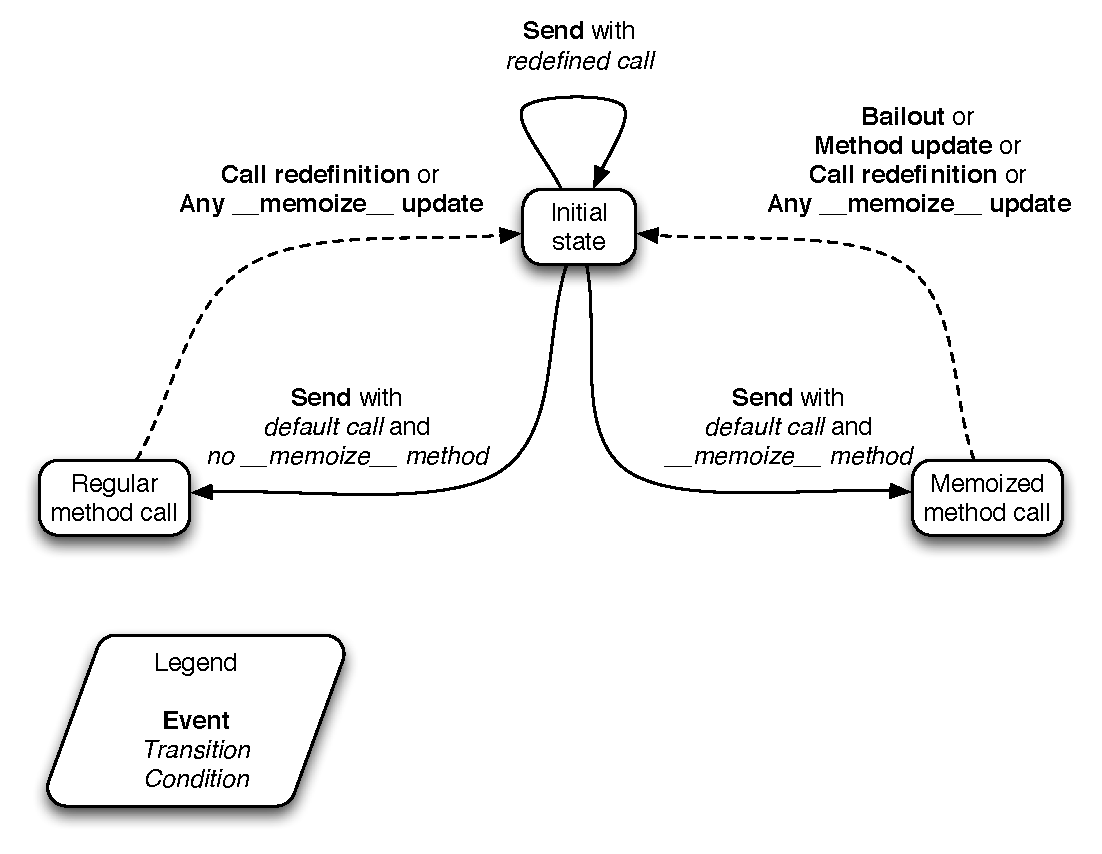
\includegraphics[width=0.8\textwidth]{figures/cacheStates}
\caption{\label{fig:CacheStates} Cache states and transitions}
\end{center}
\end{figure}

\begin{table}[!hbt]
\caption{Cache events}
\centering

\begin{tabular}{|p{.33\textwidth}|p{.33\textwidth}|}
  \hline
  Cache Events & Explanation \\
  \hline \hline
  \tbbox{Send} & 
    \tbbox{
    A message is sent to a receiver object.
    } \\
  \hline
  \tbbox{Call redefinition} & 
    \tbbox{
    The \kw{call} method on \kw{Function.prototype} is redefined.
    } \\
  \hline
  \tbbox{Any memoized redefinition} & 
    \tbbox{
    Any \kw{__memoize__} method is being redefined.
    } \\
  \hline
  \tbbox{Bailout} & 
    \tbbox{
    A run-time invariant has been violated.
    } \\
  \hline
  \tbbox{Method update} & 
    \tbbox{
    An object's method is being updated.
    } \\
  \hline
\end{tabular}

\label{tb:CacheEvents}
\end{table}

\begin{table}[htb]
\caption{Cache transition conditions}
\centering

\begin{tabular}{|p{.33\textwidth}|p{.33\textwidth}|}
  \hline
  Cache Transition Condition & Explanation \\
  \hline \hline
  \tbbox{Default call} & 
    \tbbox{
    \kw{Function.prototype call} method is the same as the one initially supplied.
    } \\
  \hline
  \tbbox{Redefined call} & 
    \tbbox{
    \kw{Function.prototype call} method is different than the one initially supplied.     
    } \\
  \hline
  \tbbox{No \kw{__memoize__} method} & 
    \tbbox{
    No method named \kw{__memoize__} has been found on the method to be called.
    } \\
  \hline
  \tbbox{\kw{__memoize__} method} & 
    \tbbox{
    A method named \kw{__memoize__} has been found on the method to be called.
    } \\
  \hline
\end{tabular}

\label{tb:CacheTransitionConditions}
\end{table}

\FloatBarrier
\section{Object representation}
\label{sec:ObjectRepresentation}

The object representation in a virtual machine is a core aspect that has a
major influence on its flexibility and performance. The following object
representation has been designed to encapsulate the invariants of our
implementation while enabling piggybacking on the underlying VM inline caches
for performance. We believe that our particular usage of the underlying object
model dynamism is new and could serve as a basis for other language
implementations seeking performance on modern JS VMs.

Two insights led to the current design. First, on a well optimized VM, the most
efficient implementation of a given operation in a metacircular implementation
is frequently the exact same operation performed by the host VM. Second, method
calls on JavaScript VMs are usually really fast. Therefore, Photon provides
operations as method calls on objects whose internal representation is as close
as possible to the host object being implemented. 

The core idea is to associate a proxy object to every object in the system and
have the proxy prototype point to the parent object's proxy. Photon optimizes
the object representation operations at runtime by attaching specialized
methods at the appropriate places on the proxy prototype chain.

The object representation is presented for native object types. A refinement is
presented for special objects to preserve performance. We then see how the
object representation is used to specialize methods for the number of arguments
found at their call site. 

\subsection{Representation for objects}

The first and simplest object type in JavaScript is the object. It has
properties and a prototype. A proxy object has a reference to the native object
to intercept every operation that goes to the object. The prototype chain of
proxies mirrors the object prototype chain. A JavaScript implementation, with
\kw{Object.prototype}, as the root of all objects, is illustrated in
Figure~\ref{fig:BasicRepresentation}.

\begin{figure}[htb]
\begin{center}
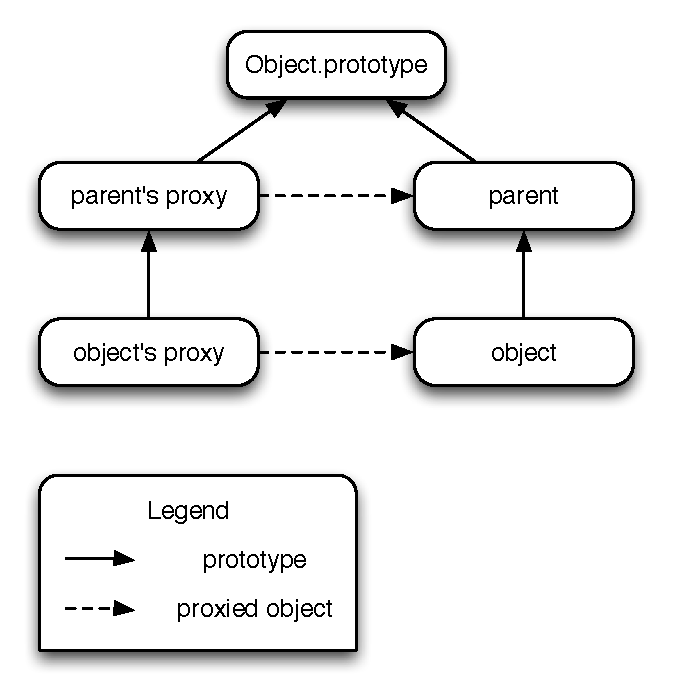
\includegraphics[scale=0.75]{figures/objectRepresentation}
\caption{\label{fig:BasicRepresentation} Representation for objects}
\end{center}
\end{figure}

An advantage of this representation is that property accesses can be
implemented directly as a native property access to the proxied object. It
allows the host VM to do lookup caching. It even works for reified root
objects, in this example, by considering \kw{parent} the \kw{Object.prototype}
of all objects of the metacircular VM.

However, it does not work well with native types that can be created literally
such as arrays, functions and regular expressions. These would require their
prototype to be changed to another object at the creation site, ruining
structural invariants assumed by the host VM. For those objects, the original
native prototype is maintained and in cases where a lookup needs to be
performed, it is done explicitly through the proxy prototype chain. This is
illustrated with arrays in Figure~\ref{fig:SpecialRepresentation}.

\begin{figure}[htb]
\begin{center}
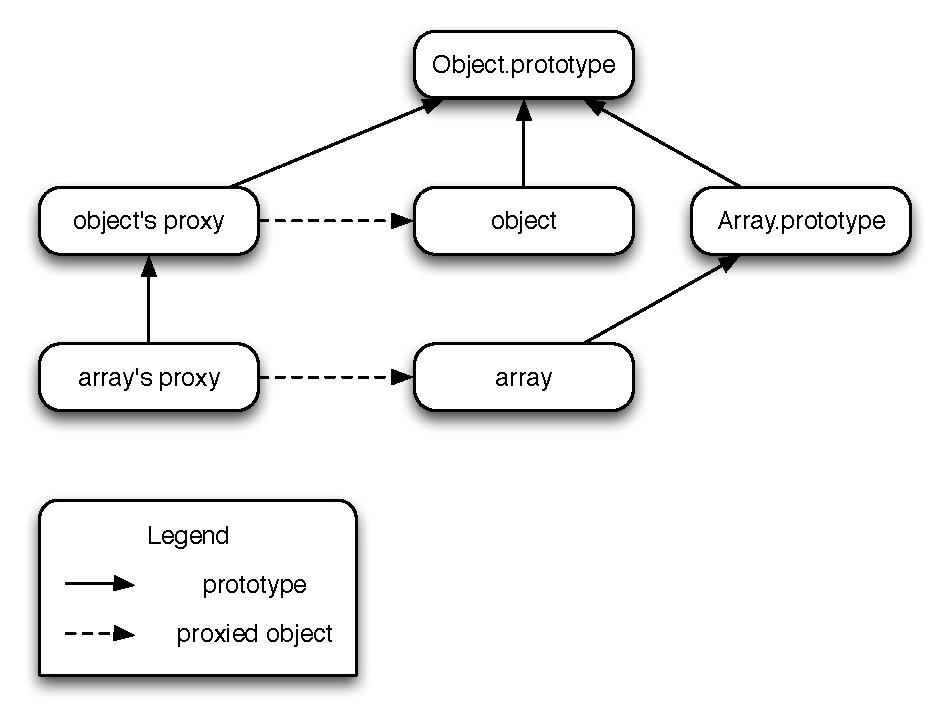
\includegraphics[scale=0.75]{figures/specialRepresentation}
\caption{\label{fig:SpecialRepresentation} Representation for special objects}
\end{center}
\end{figure}

Given this structural representation for all object types, we can now define
all object operations as methods on proxy objects as explained in
Table~\ref{tb:ObjectRepresentationOperations}. Remark that given the current
JavaScript \textit{de facto} standard of accessing the prototype object with
the \kw{__proto__} name, if proper care is not taken in the property access
method, the proxied object will be returned instead of the expected proxy object of
the parent.~\footnote{For this particular reason, we would advocate for
implementations to expose the prototype of an object through a method call
instead of a property. We could still preserve backward compatibility for
literal object definitions but once the object is created, the prototype should
not be accessible or modifiable through the \kw{__proto__} property.}

\begin{table}[htb]
\caption{Object representation operations and their interface}
\centering

\begin{tabular}{|p{.25\textwidth}|p{.33\textwidth}|p{.33\textwidth}|}
  \hline
  Operation & Explanation & Interface \\
  \hline \hline
  \tbbox{Property access} & 
    \tbbox{
        Retrieving the value of a property that might exist or not.\\
        Ex: \kw{obj.foo}  
    } &
    \tbbox{
        \kw{get(name)}\\
        Ex: \kw{obj.get("foo")}
    } \\
  \hline
  \tbbox{Property assignation} & 
    \tbbox{
        Creating or updating a property.\\
        Ex: \kw{obj.foo=42} 
    } &
    \tbbox{
        \kw{set(name, value)}\\
        Ex: \kw{obj.set("foo",42)}
    } \\
  \hline
  \tbbox{Property deletion} &
    \tbbox{
        Deleting a property that might exist or not.\\
        Ex: \kw{delete obj.foo}
    } &
    \tbbox{
        \kw{delete(name)}\\
        Ex: \kw{obj.delete("foo")}
    } \\
  \hline
  \tbbox{Property test} & 
    \tbbox{
        Test if a property name is present or not. Ex:\\
        \kw{obj.hasOwnProperty("foo")}  
    } &
    \tbbox{
        \kw{has(name)} \\
        Ex: \kw{obj.has("foo")}
    } \\
  \hline
  \tbbox{Object creation} & 
    \tbbox{
        Creating an object from a parent object.\\
        Ex: \kw{Object.create(parent)} 
    } &
    \tbbox{
        \kw{create()}\\
        Ex: \kw{parent.create()}
    } \\
  \hline
  \tbbox{Call} & 
    \tbbox{
        Call the object as a function.\\
        Ex: \kw{fun()} 
    } &
    \tbbox{
        \kw{call(rcv, ..args)}\\
        Ex: \kw{fun.call(global)}
    } \\
  \hline
  \tbbox{Box} & 
    \tbbox{
        Returns the proxy of an object if applicable.
    } &
    \tbbox{
        \kw{box()}\\
        Ex: \kw{obj.box()}
    } \\
   \hline
  \tbbox{Unbox} & 
    \tbbox{
        Returns the proxied object.
    } &
    \tbbox{
        \kw{unbox()}\\
        Ex: \kw{obj.unbox()}
    } \\
   \hline
  \tbbox{Prototype access} & 
    \tbbox{
        Returns the prototype of an object.\\
        Ex: \kw{obj.__proto__}
    } &
    \tbbox{
        \kw{getPrototype()}\\
        Ex: \kw{obj.getPrototype()}
    } \\
   \hline
  \tbbox{Prototype update} & 
    \tbbox{
        Sets the prototype of an object.\\
        Ex: \kw{obj.__proto__ = parent}
    } &
    \tbbox{
        \kw{setPrototype(parent)}\\
        Ex: \kw{obj.setPrototype(parent)}
    } \\
   \hline
\end{tabular}

\label{tb:ObjectRepresentationOperations}
\end{table}


Proxies can adapt to dynamic circumstances by adding specialized methods at run
time, which can be used for performance gains. The next section shows how
Photon exploits this possibility to specialize operations to a fixed number of
arguments. To avoid name clashing and ease reading we adopt the convention that
specialized methods share the same prefix as basic methods with the type or
value information and or number of arguments following in the name.

\FloatBarrier

\subsection{Fixed arguments number specialization}

The object representation design does not require a special calling convention
for functions. However, for maximum performance gains in JavaScript, we would
like to avoid using the \kw{call} and \kw{apply} native methods. We can do it
by globally rewriting every function to explicitly pass the receiver object. This
way, a specialized call operation can simply pass the references to the native
function. An example implementation for a \kw{call} operation, specialized for
one argument in addition to its receiver, is:

\jsfile{listings/function-call-example.js}

Specializing one proxy operation requires to specialize \textit{all} objects
for that particular operation to ensure that whatever receiver, function or
object is called at a given site, a proper operation is supplied. Fortunately,
the object-oriented nature of our chosen representation makes it easy. Only
root proxies need to have an additional method and all other proxies  then
implement the specialized operation.

%\subsection{Type or value specialization}
%
%In the same way, we can specialize an operation for a known value. For
%example, suppose we would like an optimized operation that accesses a constant 
%property name. A proper specialized method could be written:
%
%\jsfile{listings/proxy-operation-specialization.js}
%
%Notice that a method that falls back to the general case is provided to the
%root object to add support to all other proxies. The same idiom can be used for
%type specialization instead of value.

%\subsection{Note}
%
%The idea of mirroring the object prototype chain in the proxy prototype chain
%came as a surprise during the implementation of the VM and was partially
%exploited to obtain our current performance results. However, because of time
%constraints and not strict necessity to our thesis, an extensive empirical
%study of its performance characteristics and the exploitation of every
%optimization opportunity is yet to be performed. We decided to present the idea
%here first, before it was fully fleshed-out, to both claim originality and give
%the reader a primer on its possibilities. In the remainder of this
%dissertation, we will only present aggregate performance results for our VM on
%common benchmarks without trying to extract the contribution provided by this
%object representation. The reader should keep in mind that the arguments number
%specialization for the \kw{call} method is performed but not the
%object-representation operation specialization. An exhaustive empirical study
%should be the focus of a subsequent publication.

\section{Compilation example}

To wrap up and see how those different elements work together in practice,
let's finish with a brief compilation example. We use the following example:

\jsfile{listings/compilation-example.js}

In this example, an anonymous function is called right after being created to
provide a lexical scope, which means that the \kw{o} and \kw{i} variables are
local to the function. In this scope, we create an \kw{o} empty object, which
has the root object of the metacircular VM for prototype. Then, this object is
extended with a \kw{foo} method. This method returns the \kw{bar} property of
the receiver object. We then create and initialize the \kw{bar} property of the
\kw{o} object. Finally, we call the \kw{foo} method two times to give it the
chance to specialize the call site, both of the \kw{foo} call and the \kw{bar}
property access inside the \kw{foo} method.

We first see how compiling this example to message sends uses the inline
caching idiom. The compiled code has been weaved with the original code in
comments to allow the reader to follow easily:

\jsfile{listings/compilation-example-compiled.js}

\newpage

In addition to what has been discussed in this chapter, this example exhibits
additional implementation details:
\begin{itemize}
    \item \textit{Type information in data caches}: During compilation, known
    types which directly correspond to abstract syntax tree nodes are preserved.
    It allows the runtime to exploit stable information. For example, in
    \kw{dataCache1}, the \kw{"string"} type allows the runtime to know the
    property access is to a constant string name.    
    \item \textit{Root objects are different from the host root objects}:
    \kw{root.function}, \kw{root.object} and \kw{root.global} virtualize the
    object model root objects to avoid interference with the host objects.
    \item \textit{Functions have an extra \kw{\$closure} parameter}: This extra
    parameter is used to pass the proxy to the function to the code or
    dataCache information for the implementation to send the cache state to the
    cache function behavior.
\end{itemize}

Apart from those additional details, the compilation conforms to the
explanation given in this chapter. The environment is used as such, without
reification, objects are proxied or created from object representation methods.

After execution, the inline caches at \kw{codeCache1} and \kw{codeCache5} are
respectively in a memoized state and a regular method call state, which
correspond to the following behaviors: 

\jsfile{listings/compilation-example-compiled-specialized.js}

In the last case, we can see that the \kw{call} method has been specialized for
no arguments, exploiting optimization opportunities offered by our object
representation. This example therefore summarizes the unification of object
model operations to message sends, their efficient implementation and a novel
object representation that can dynamically adapt itself to information
available at runtime.

The next chapter shows how we can use the added flexibility for instrumentation
and runtime invariant monitoring.


